\chapter{Barrier Transport and Space-Charge-Limited Current}
\label{ch:barrier-space-charge-transport}

Drift and diffusion describe carriers that remain inside a band.  Interfaces and
strong injection introduce different transport controls.  Thermionic emission
selects carriers above a barrier, tunneling transmits wave amplitude through a
barrier, and space charge couples injected density back to the electric field
\cite[Chap.~2]{szeLee2012}.

\section{Notation and units}

\begin{center}
\small
\begin{tabularx}{\textwidth}{@{}lX@{}}
\toprule
Symbol & Meaning and SI unit unless stated otherwise \\
\midrule
$q,\kb,T$ & Positive elementary charge, Boltzmann constant, and absolute temperature. \\
$E_C,E_F$ & Conduction-band edge and Fermi energy, measured in joules or electron-volts under one consistent convention. \\
$\chi,V_n,\Phi_B$ & Electron affinity, conduction-band-to-Fermi-level separation, and emission barrier, each expressed in volts so multiplication by $q$ gives energy. \\
$N_C,n_{\mathrm{th}}$ & Conduction-band effective density of states and thermionically eligible electron density, measured in inverse cubic meters. \\
$A^*$ & Effective Richardson constant, measured in amperes per square meter-kelvin squared. \\
$J_{\mathrm{th}}$ & Thermionic current density, measured in amperes per square meter. \\
$U_0,E$ & Rectangular-barrier energy and incident carrier energy, measured in joules or electron-volts under one consistent convention. \\
$d,\kappa,m^*,\hbar$ & Barrier width in meters, evanescent decay constant in inverse meters, effective mass in kilograms, and reduced Planck constant in joule-seconds. \\
$\mathcal T(E)$ & Dimensionless transmission probability at energy $E$. \\
$x_i,\Delta x,N$ & Finite-difference grid point, grid spacing in meters, and number of grid points. \\
$t_0,\bm H,\bm G^r$ & Finite-difference hopping energy, Hamiltonian matrix, and retarded Green matrix. \\
$\Sigma_{L,R},\Gamma_{L,R}$ & Lead self-energies and broadenings, measured in joules. \\
$\rho,n,p,N_D^+,N_A^-$ & Charge density in coulombs per cubic meter and mobile or ionized carrier densities in inverse cubic meters. \\
$\phi,\mathcal E$ & Electrostatic potential in volts and one-dimensional electric-field magnitude in volts per meter. \\
$J,\mu,\epsilon_s$ & Current density, mobility, and semiconductor permittivity in amperes per square meter, square meters per volt-second, and farads per meter. \\
$V,L,v_s$ & Applied voltage in volts, layer length in meters, and saturation velocity in meters per second. \\
\bottomrule
\end{tabularx}
\end{center}

\section{Thermionic emission}

The electron affinity $\chi$ is the energy separation, expressed in volts,
between the conduction-band edge and the vacuum level.  If
$E_C-E_F=qV_n$, an electron must acquire energy $q(\chi+V_n)$ to leave an
isolated n-type semiconductor.  In the nondegenerate limit, the population
above that barrier scales as
\begin{equation}
  n_{\mathrm{th}}
  \propto N_C
  \exp\left[-\frac{q(\chi+V_n)}{\kb T}\right].
  \label{eq:thermionic-tail-density}
\end{equation}
The exponential factor dominates the emission probability.  A modest change in
barrier energy therefore changes the emitted population by orders of
magnitude.

The directed flux contains an additional velocity moment.  For a parabolic
band and an ideal absorbing interface, the current takes the Richardson form
\begin{equation}
  J_{\mathrm{th}}=A^*T^2
  \exp\left(-\frac{q\Phi_B}{\kb T}\right),
  \label{eq:richardson-emission}
\end{equation}
where $A^*$ contains the transport effective mass and $\Phi_B$ is the relevant
barrier in volts.  Interface reflection, image-force lowering, tunneling, and
nonparabolic bands modify this ideal law.

\section{Quantum tunneling through a barrier}

Consider a rectangular barrier with energy height $U_0$ and width $d$.  For
carrier energy $0<E<U_0$, the wavefunction inside the barrier contains
evanescent terms with decay constant
\begin{equation}
  \kappa=\frac{\sqrt{2m^*(U_0-E)}}{\hbar}.
  \label{eq:rectangular-kappa}
\end{equation}
Continuity of the wavefunction and its derivative gives
\begin{equation}
  \boxed{
  \mathcal T(E)=
  \left[
    1+\frac{U_0^2\sinh^2(\kappa d)}{4E(U_0-E)}
  \right]^{-1}.
  }
  \label{eq:rectangular-barrier-transmission}
\end{equation}
When $\kappa d\gg1$,
\begin{equation}
  \mathcal T(E)\propto e^{-2\kappa d}.
  \label{eq:tunneling-wkb-scaling}
\end{equation}
The transmission increases for a thinner barrier, a lower barrier, a higher
incident energy, or a smaller effective mass.  Tunneling and thermionic
emission therefore sample different parts of the same energy landscape:
thermionic carriers pass over a barrier, while tunneling carriers retain finite
transmission below it.

\section{Space charge from injected carriers}

The semiconductor charge density is
\begin{equation}
  \rho=q(p-n+N_D^+-N_A^-).
  \label{eq:semiconductor-space-charge-density}
\end{equation}
Charge neutrality makes this quantity nearly zero in a uniform bulk region.
Strong injection breaks that cancellation.  For electron injection with
$n\gg N_D^+$ and negligible holes, the charge magnitude is $qn$ and Poisson's
equation links the carrier density to the field gradient.

Assume a one-dimensional layer of length $L$, constant mobility, negligible
diffusion, and an injecting contact at which the field vanishes.  Current and
Poisson equations give
\begin{equation}
  J=qn\mu\mathcal E,
  \qquad
  \frac{\dd\mathcal E}{\dd x}=\frac{qn}{\epsilon_s}.
  \label{eq:sclc-current-poisson}
\end{equation}
Eliminating $n$ yields
\begin{equation}
  \mathcal E\frac{\dd\mathcal E}{\dd x}
  =\frac{J}{\epsilon_s\mu}.
  \label{eq:sclc-field-equation}
\end{equation}
The ohmic injecting-contact condition is $\mathcal E(0)=0$.  Integration gives
\begin{equation}
  \mathcal E(x)
  =\sqrt{\frac{2Jx}{\epsilon_s\mu}}.
  \label{eq:mott-gurney-field-profile}
\end{equation}
The applied voltage is the field integral,
\begin{equation}
  V=\int_0^L\mathcal E(x)\,\dd x
  =\frac23\sqrt{\frac{2J}{\epsilon_s\mu}}L^{3/2}.
  \label{eq:mott-gurney-voltage-integral}
\end{equation}
Solving for $J$ produces the trap-free Mott--Gurney law
\begin{equation}
  \boxed{
  J=\frac98\epsilon_s\mu\frac{V^2}{L^3}.
  }
  \label{eq:mott-gurney-law}
\end{equation}
The quadratic voltage dependence distinguishes space-charge-limited current
from an ohmic current proportional to $V$.

When carrier speed has reached a field-independent saturation value $v_s$,
$J=qn v_s$.  Poisson's equation then gives a linear field:
\begin{equation}
  \mathcal E(x)=\frac{Jx}{\epsilon_s v_s},
  \qquad
  V=\frac{JL^2}{2\epsilon_s v_s}.
  \label{eq:saturated-sclc-field-profile}
\end{equation}
Therefore
\begin{equation}
  \boxed{
  J=2\epsilon_s v_s\frac{V}{L^2}.
  }
  \label{eq:saturated-sclc-law}
\end{equation}
Velocity saturation changes both the voltage exponent and the length scaling.
Traps introduce additional stored charge and produce other exponents or
thresholds.

\begin{figure}[htbp]
  \centering
  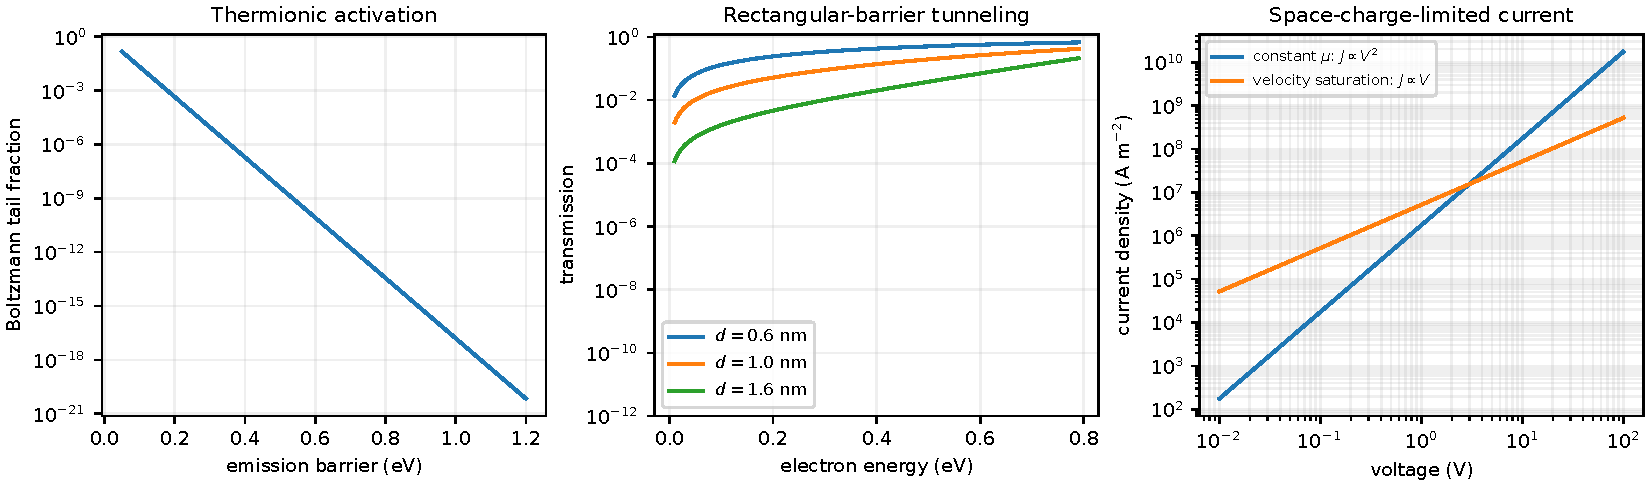
\includegraphics[width=\textwidth]
    {figures/transport-barriers-space-charge.pdf}
  \caption{Thermionic activation by the Boltzmann tail, tunneling through
  finite-width barriers, and the distinct voltage scalings of constant-mobility
  and velocity-saturated space-charge-limited current.\figurenotebookmark}
  \label{fig:transport-barriers-space-charge}
\end{figure}
\figurenotebooktext{figures/14_barrier-space-charge-transport/fig_14_01.ipynb}

\section{Finite-difference barrier and space-charge calculations}

The closed-form barrier and space-charge laws provide validation targets for
numerical methods that also apply to nonrectangular potentials and nonuniform
charge.  Three finite-difference problems are treated separately: the open
quantum barrier, Poisson electrostatics for prescribed charge, and the nonlinear
space-charge field with unknown current.

\subsection{Open-boundary Schrödinger equation}

On a cell-centered grid inside the barrier, the second derivative is
\begin{equation}
  \left.\frac{\dd^2\psi}{\dd x^2}\right|_i
  \simeq
  \frac{\psi_{i-1}-2\psi_i+\psi_{i+1}}{\Delta x^2}.
  \label{eq:barrier-second-difference}
\end{equation}
Define
\begin{equation}
  t_0=\frac{\hbar^2}{2m^*\Delta x^2}.
  \label{eq:barrier-fd-hopping}
\end{equation}
The finite-difference Hamiltonian has diagonal entries $2t_0+U_i$ and nearest-
neighbor entries $-t_0$.  Setting the wavefunction to zero at the ends would
turn the barrier into a closed box and eliminate transmitted flux.  Transport
requires open boundaries connected to semi-infinite leads.

A zero-potential discrete lead has dispersion
\begin{equation}
  E=2t_0[1-\cos(k\Delta x)].
  \label{eq:discrete-lead-dispersion}
\end{equation}
Its retarded boundary self-energy and broadening are
\begin{equation}
  \Sigma=-t_0e^{ik\Delta x},
  \qquad
  \Gamma=-2\operatorname{Im}\Sigma.
  \label{eq:discrete-lead-self-energy}
\end{equation}
With one lead attached to each end, the open retarded Green matrix is
\begin{equation}
  \bm G^r(E)=
  \left[E\bm I-\bm H-\Sigma_L-\Sigma_R\right]^{-1}.
  \label{eq:barrier-retarded-green-matrix}
\end{equation}
Only the end-to-end element is required in one dimension:
\begin{equation}
  \boxed{
  \mathcal T_{
m FD}(E)
  =\Gamma_L\Gamma_R\left|G^r_{1N}(E)\right|^2.
  }
  \label{eq:barrier-fd-transmission}
\end{equation}
This formulation preserves incoming and outgoing flux and converges to
\cref{eq:rectangular-barrier-transmission} as $\Delta x\to0$.

\subsection{Poisson equation for prescribed charge}

For electrostatic potential $\phi$, Poisson's equation is
\begin{equation}
  \frac{\dd^2\phi}{\dd x^2}=-\frac{\rho(x)}{\epsilon_s}.
  \label{eq:poisson-potential-one-dimensional}
\end{equation}
At an interior node,
\begin{equation}
  \phi_{i-1}-2\phi_i+\phi_{i+1}
  =-\frac{\Delta x^2}{\epsilon_s}\rho_i.
  \label{eq:poisson-centered-difference}
\end{equation}
Dirichlet contact potentials replace the first and last matrix rows.  The
result is a tridiagonal linear system.  A uniform charge with
$\phi(0)=\phi(L)=0$ has the analytic parabola
\begin{equation}
  \phi(x)=\frac{\rho}{2\epsilon_s}x(L-x),
  \label{eq:uniform-charge-potential}
\end{equation}
which tests both the sign convention and second-order stencil.

\subsection{Current-constrained nonlinear space charge}

For unipolar injection, eliminate the density from $J=qn v(\mathcal E)$ and
Poisson's equation:
\begin{equation}
  \frac{\dd\mathcal E}{\dd x}
  =\frac{J}{\epsilon_s v(\mathcal E)}.
  \label{eq:general-space-charge-field-equation}
\end{equation}
The current $J$ is not supplied; it is fixed by the applied voltage.  At each
cell midpoint, the finite-difference residual is
\begin{equation}
  F_i=\mathcal E_{i+1}-\mathcal E_i
  -\frac{\Delta x\,J}
  {\epsilon_s v[(\mathcal E_i+\mathcal E_{i+1})/2]}.
  \label{eq:sclc-fd-cell-residual}
\end{equation}
The unknown vector contains all nodal fields and $J$.  It is closed by
\begin{equation}
  \mathcal E_0=0,
  \qquad
  \sum_i\frac{\mathcal E_i+\mathcal E_{i+1}}2\Delta x=V.
  \label{eq:sclc-fd-constraints}
\end{equation}
A bounded nonlinear least-squares solver enforces nonnegative field and current.
Using $v=\mu\mathcal E$ recovers the square-root field profile and Mott--Gurney
current.  Using $v=v_s$ recovers the linear field profile and the saturated
current law.

\begin{center}
\small
\begin{tabular}{@{}lll@{}}
\toprule
Numerical check & Result & Acceptance condition \\
\midrule
Barrier transmission relative $L_2$ error, $N=100$ & $5.88\times10^{-5}$ & below $10^{-4}$ \\
Uniform-charge Poisson error & $7.61\times10^{-15}$ & below $10^{-10}$ \\
Mott--Gurney current relative error, $N=81$ & $8.53\times10^{-4}$ & below $10^{-3}$ \\
Constant-velocity current relative error & $6.67\times10^{-11}$ & below $10^{-8}$ \\
\bottomrule
\end{tabular}
\end{center}

\begin{figure}[htbp]
  \centering
  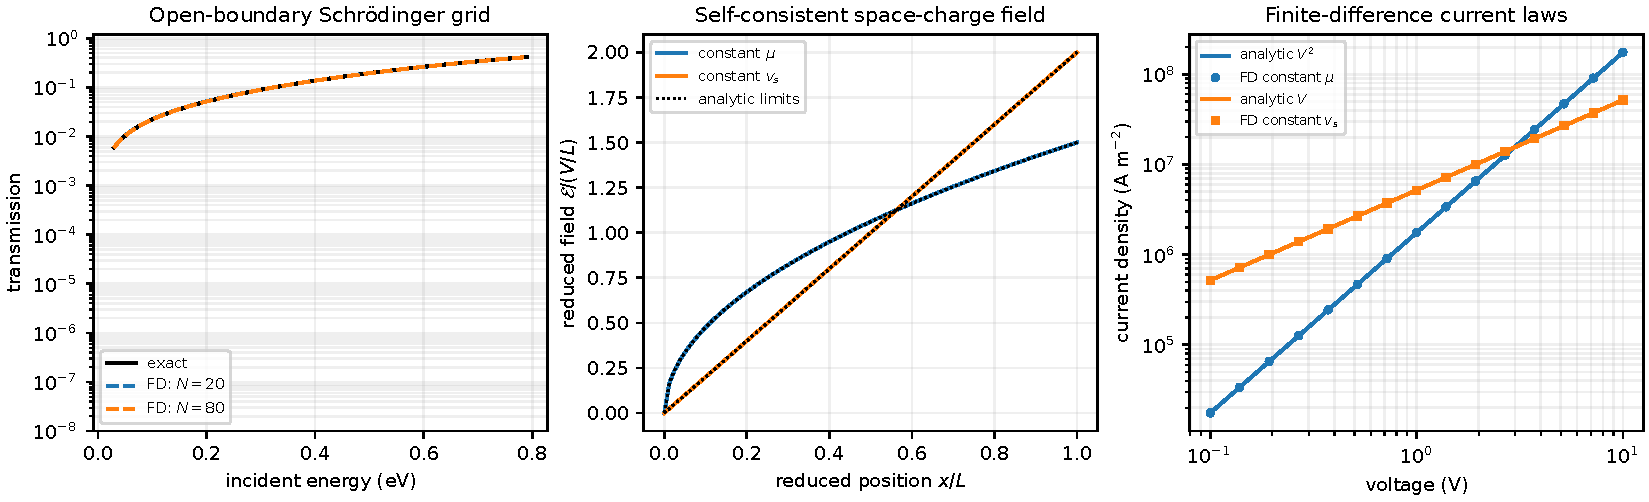
\includegraphics[width=\textwidth]
    {figures/transport-barrier-sclc-numerics.pdf}
  \caption{Convergence of open-boundary finite-difference tunneling to the exact
  rectangular-barrier result, numerical space-charge field profiles in the
  constant-mobility and constant-velocity limits, and recovery of their
  quadratic and linear current--voltage laws.\figurenotebookmark}
  \label{fig:transport-barrier-sclc-numerics}
\end{figure}
\figurenotebooktext{figures/14_barrier-space-charge-transport/fig_14_01.ipynb}

\section{Range of validity}

The thermionic law assumes a thermalized nondegenerate population and an ideal
interface.  The rectangular-barrier result and its finite-difference model are
one-dimensional, coherent, elastic, and constant-mass.  The quantum grid must
resolve both the lead wavelength and the evanescent decay length; its discrete
lead band must contain every incident energy.  The Mott--Gurney calculation
assumes trap-free injection, one carrier type, negligible diffusion, and an
ohmic contact with $\mathcal E(0)=0$.  A nonohmic contact replaces that boundary
condition and changes the current.  Real interfaces combine thermionic
emission, field lowering, tunneling, trapping, and contact resistance.  Their
relative importance is determined by barrier shape, temperature, field, and
scattering length.

\section{Chapter summary}

Thermionic emission depends exponentially on barrier energy relative to
thermal energy.  Quantum tunneling depends exponentially on barrier width and
evanescent decay constant.  Open-boundary finite differences reproduce the
exact rectangular-barrier transmission and extend to arbitrary barrier shapes.
Centered finite differences solve Poisson's equation for nonuniform charge.
Under strong injection, simultaneous solution of the field profile and voltage
constraint produces space-charge-limited current.  Constant mobility yields
$J\propto V^2/L^3$, while velocity saturation yields $J\propto V/L^2$.
